\subsection{Ca sử dụng mời bạn bè tham gia chuyến đi}
\noindent Ca sử dụng này mô tả cách người dùng mời bạn bè của họ tham gia vào một chuyến đi công khai mà họ đã tạo hoặc đang tham gia. Hệ thống sẽ gửi thông báo mời đến những người được chọn. Bảng~\ref{tab:uc_invite_friend_spec} trình bày chi tiết đặc tả ca sử dụng, bao gồm luồng sự kiện chính, luồng thay thế, các điều kiện và yêu cầu liên quan. Các biểu đồ hoạt động, quan hệ (Bảng~\ref{tab:uc_invite_friend_diagrams}) và tuần tự (Hình~\ref{fig:3-3-14-sequence-diagram}) minh họa rõ hơn về quy trình và tương tác hệ thống khi mời bạn bè.
% \vspace{0.5cm} % Adjust spacing if needed

% Use longtable environment
% Need \usepackage{longtable} and \usepackage{calc} in preamble
\begin{longtable}{| p{4cm} | p{\dimexpr\linewidth-4cm-4\tabcolsep} |} % Adjust widths as needed
    \caption{Đặc tả ca sử dụng mời bạn bè tham gia chuyến đi} % Caption inside longtable (no period)
    \label{tab:uc_invite_friend_spec} \\ % Label after caption

    \hline
    \textbf{Mô tả} & Người dùng có thể mời bạn bè tham gia chuyến đi của mình hoặc mình tham gia. \\
    \hline
    \endfirsthead % Header for the first page

    % No \endhead content needed

    % No \endfoot content needed

    \hline % Footer for the last page
    \endlastfoot

    % --- Table Content ---
    \textbf{Luồng cơ bản} & 1. Người dùng chọn một chuyến đi muốn mời bạn bè. \newline
                           2. Hệ thống lấy dữ liệu chi tiết của chuyến đi và hiển thị. \newline
                           3. Người dùng bấm "Mời thành viên". \newline
                           4. Hệ thống điều hướng sang trang thêm thành viên và hiển thị thanh tìm kiếm. \newline
                           5. Người dùng nhập tên thành viên muốn mời. \newline
                           6. Hệ thống tìm kiếm và hiển thị danh sách các tài khoản phù hợp với từ khóa tìm kiếm. \newline
                           7. Người dùng chọn các tài khoản muốn mời. \newline
                           8. Hệ thống gửi thông báo mời vào chuyến đi và thông báo đã mời thành công. \\
    \hline
    \textbf{Luồng thay thế} & Người dùng được mời đã tham gia hoặc đã từ chối sẽ không được gửi thông báo tiếp. \\
    \hline
    \textbf{Tiền điều kiện} & - Người dùng đang đăng nhập và phiên đăng nhập chưa kết thúc.\newline
                           - Người dùng đã tạo hoặc tham gia ít nhất một chuyến đi. \newline
                           - Chuyến đi phải là chuyến đi công khai.\newline
                           - Trạng thái chuyến đi khác "Đã hoàn thành" và "Hủy". \\
    \hline
    \textbf{Hậu điều kiện} & - Hệ thống gửi thông báo mời vào chuyến đi cho các tài khoản được chọn. \\
    \hline
    \textbf{Yêu cầu phi chức năng} & Hệ thống gửi lời mời bạn bè dưới 1s với 1 tài khoản. \\
    % --- End Table Content ---

\end{longtable}
\vspace{0.8cm}

\begin{table}[H] % Wrap the diagrams table
    \centering
    \caption{Biểu đồ hoạt động ca sử dụng mời bạn bè tham gia chuyến đi} % Add caption (no period)
    \label{tab:uc_invite_friend_diagrams} % Add label
    \begin{tabular}{| c | c |}
        \hline
        \textbf{Biểu đồ hoạt động} & \textbf{Quan hệ} \\
        \hline
        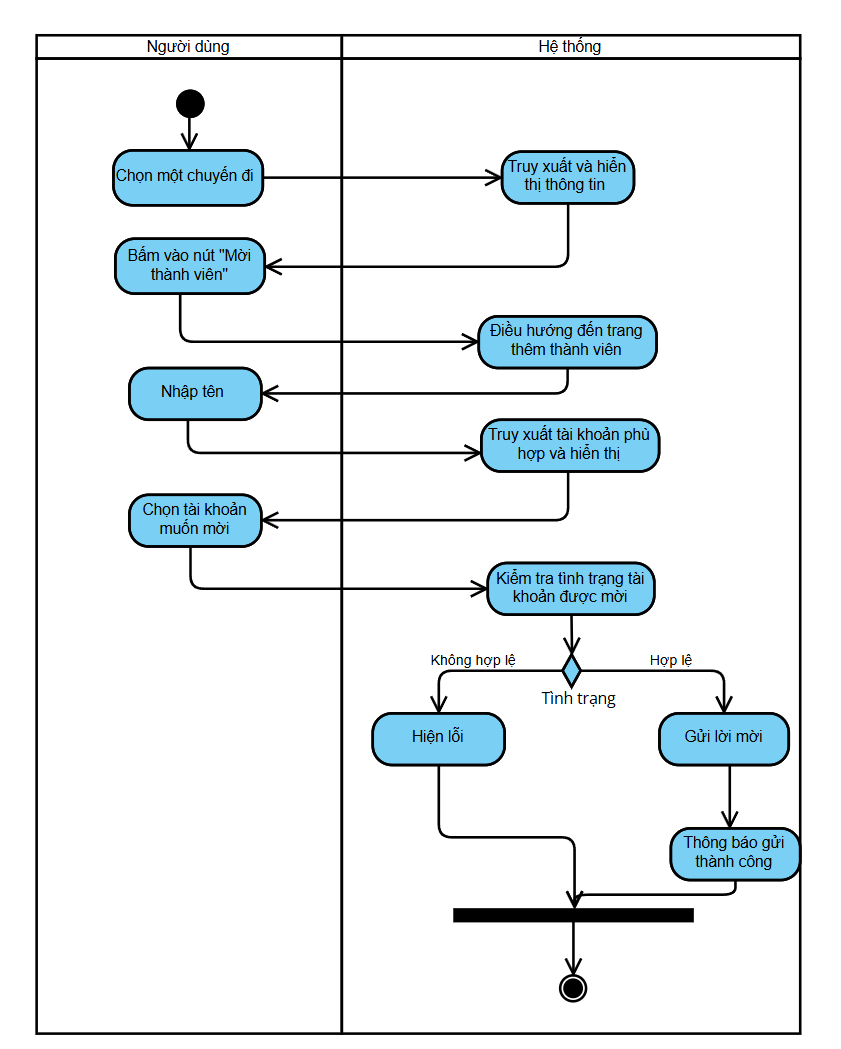
\includegraphics[width=0.5\linewidth]{figures/c3/3-3-14-ad.png} % Specified width
        &
        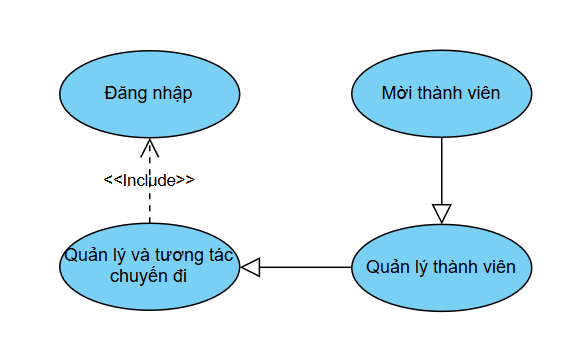
\includegraphics[width=0.45\linewidth]{figures/c3/3-3-14-rd.png} \\ % Specified width
        \hline
    \end{tabular}
\end{table}

\begin{figure}[H]
    \centering
    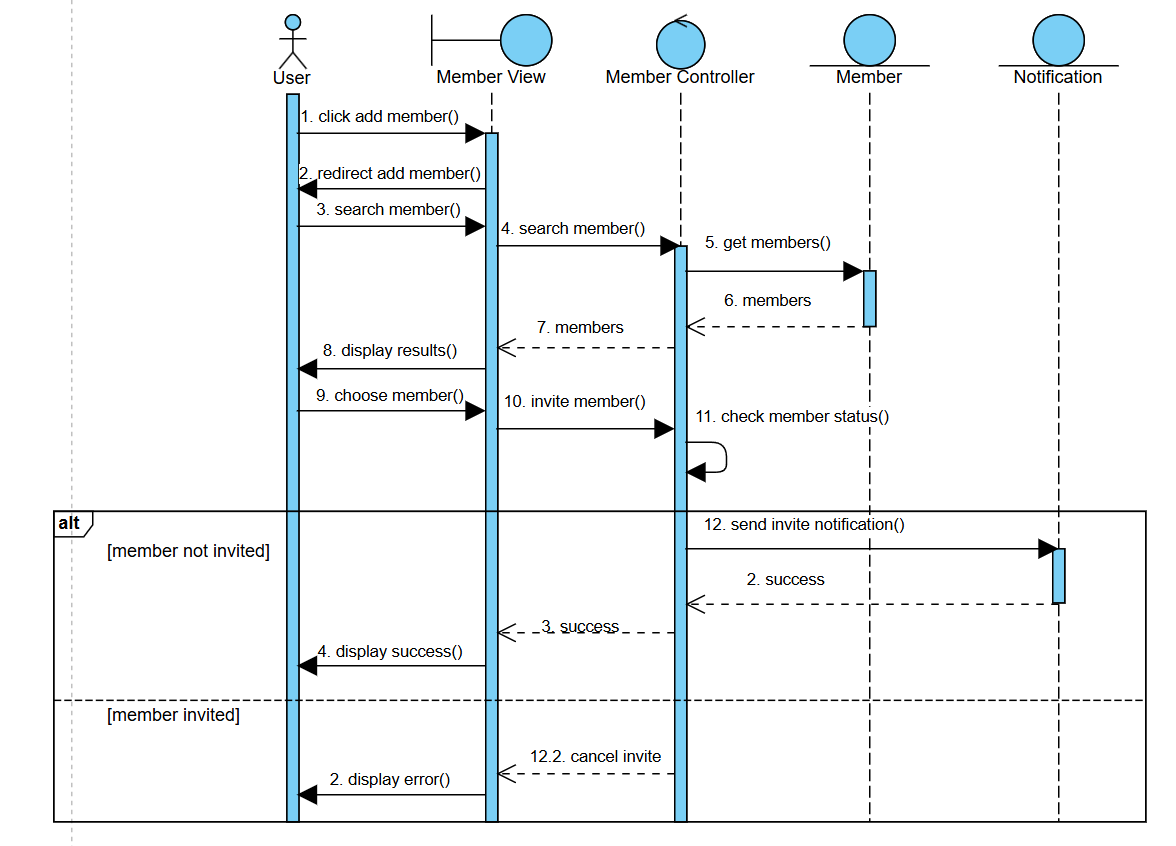
\includegraphics[width=0.85\textwidth]{figures/c3/3-3-14-sd.png} % Specified width
    \caption{Biểu đồ tuần tự ca sử dụng mời bạn bè tham gia chuyến đi.} % (no period)
    \label{fig:3-3-14-sequence-diagram}
\end{figure}